\chapter{Resultados e Discussão}
\label{cap:04}

\title{Resultados Parciais}

Os primeiros circuitos de testes foram construídos em uma Matriz de Contato (\textit{Protoboard}), de modo a facilitar ajustes e adequações de projeto. Para os experimentos foi utilizado uma lâmpada halogena, possibilitando um ambiente controlado para testes, de modo a não depender das condições climáticas ideias para efetuar o experimento. Para alterar a potência de irradiação luminosa expelida pela lâmpada sobre o painel, utilizou-se diferentes distâncias entre a lâmpada e o painel fotovoltaico. Para atestar a alteração da potência irradiada pela lâmpada sobre a superfície do painel, fez-se o uso do solarímetro.

\FloatBarrier
\begin{figure}[!htbp]
	\centering
	%scale redimensiona a figura.
	%1.5 = 150% do tamanho original
	%1 = 100% do tamanho original
	%0.20 = 20% do tamanho original
	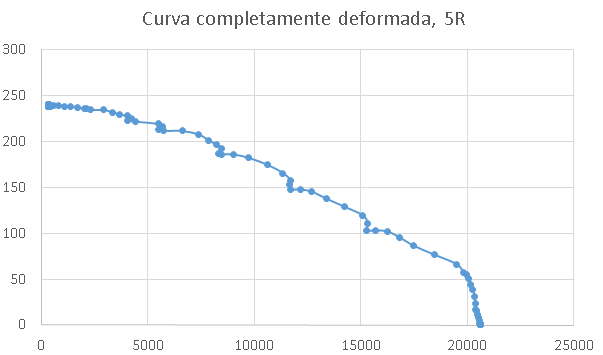
\includegraphics[scale=1]{imagens/CurvaIVdeformadaII}
	\caption{Curva IV deformada devido ao uso de um resistor de 5 Ohms. Fonte: Elaborado pelo Autor. 	}
	\label{fig:CurvaIVdeformadaII}
\end{figure}
\FloatBarrier

%//Acrescentar Imagem de Curvas Morçadas e a foto do circuito na protoboard sem o ADS ou ADC//

Os testes com dos circuitos iniciais não trouxeram os resultados esperados, fazendo com que fosse alterado o projeto. As principais alterações foram a implementação do módulo ADC (ADS1115), a alteração do valor de resistência de carga de 3 para 1 Ohm e a alteração do valor do capacitor de 1000uF para 100uF.

\FloatBarrier
\begin{figure}[!htbp]
	\centering
	%scale redimensiona a figura.
	%1.5 = 150% do tamanho original
	%1 = 100% do tamanho original
	%0.20 = 20% do tamanho original
	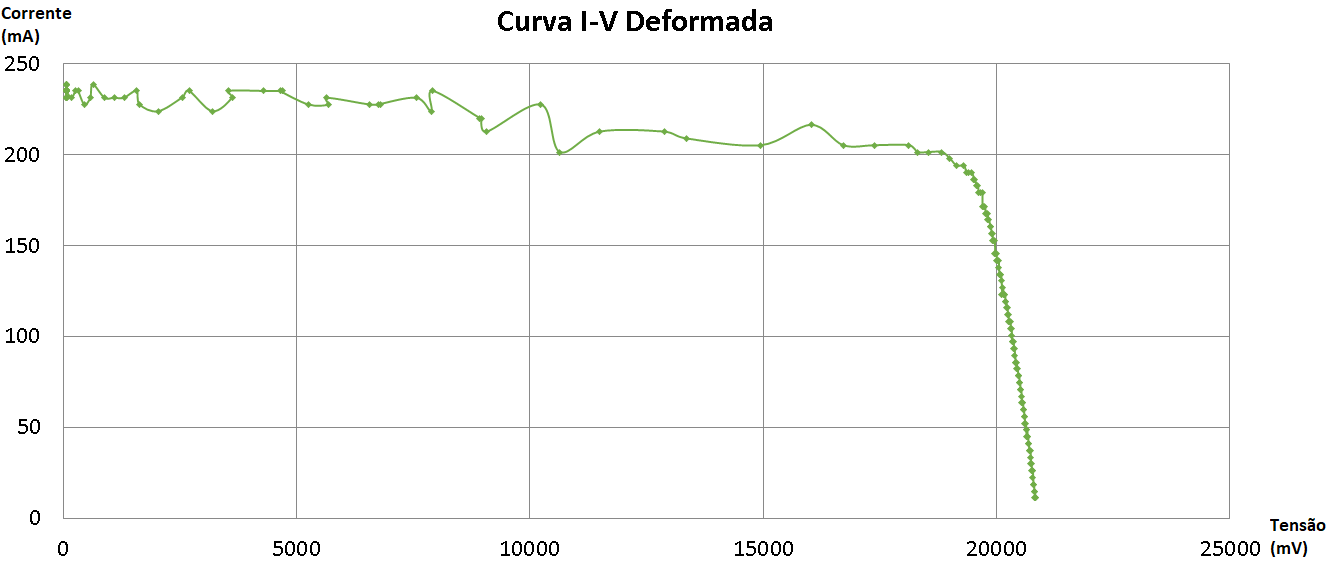
\includegraphics[scale=0.4]{imagens/CurvaIVdeformada}
	\caption{Curva IV deformada devido. Fonte: Elaborado pelo Autor. 	}
	\label{fig:CurvaDeformada}
\end{figure}
\FloatBarrier

%// Acrescentar Imagem de Curvas Morçadas e a foto do circuito na protoboard com o ADS ou ADC//

Com as alterações feitas no circuito, ainda não foi possível obter a curva ideal, de modo que foi necessário efetuar a alteração da programação, configurando diferentes resoluções do pulso de PWM de modo que foi possível traçar curvas com diferentes números de pontos de observação.

\FloatBarrier
\begin{figure}[!htbp]
	\centering
	%scale redimensiona a figura.
	%1.5 = 150% do tamanho original
	%1 = 100% do tamanho original
	%0.20 = 20% do tamanho original
	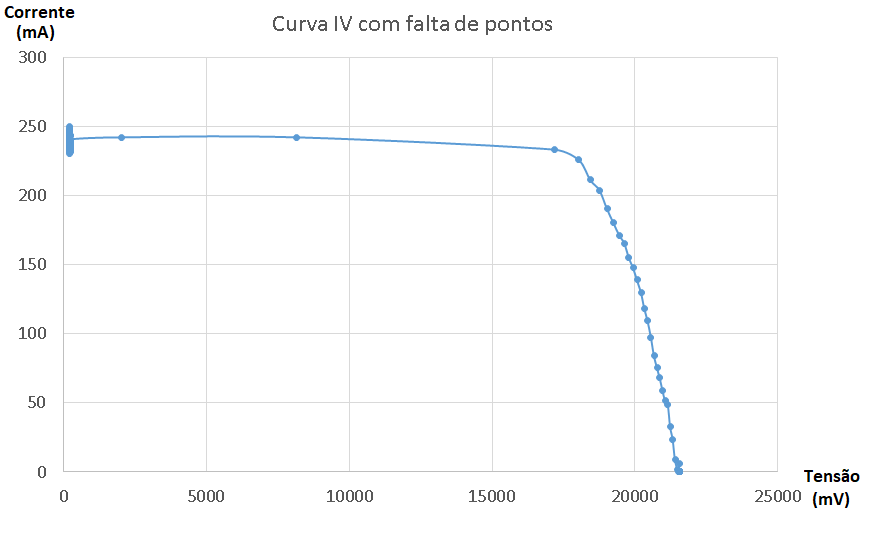
\includegraphics[scale=0.7]{imagens/CurvaIVpoucospontos}
	\caption{Curva IV com poucos pontos. Fonte: Elaborado pelo Autor. 	}
	\label{fig:Curvapoucos}
\end{figure}
\FloatBarrier

%// Acrescentar imagens de Curvas quaaase ideais só que com pouco pontos//.

Após efetuar ajustes no circuito e na programação , foi concluída a fase de teste na \textit{protoboard} obtendo exito na parte experimental. Foi possível traçar a curva I-V ideal do painel fotovoltaico e analisar seu comportamento em diferentes níveis de irradiância solar simulada.
CurvaIVpoucospontos

// Acrescentar fotos do Circuito na protoboard sendo testado (Tirar foto Logo menos), e acrescentar as curvas topzeras)

Resultados Finais:
Após concluir a fase de testes, iniciou-se a fase de confecção do circuito oficial, passando a configuração da \textit{protoboard} para uma placa de circuito impresso.... (Continua nos próximos episódios)  Texto dos resultados.